%% 
%% Copyright 2007-2025 Elsevier Ltd
%% 
%% This file is part of the 'Elsarticle Bundle'.
%% ---------------------------------------------
%% 
%% It may be distributed under the conditions of the LaTeX Project Public
%% License, either version 1.3 of this license or (at your option) any
%% later version.  The latest version of this license is in
%%    http://www.latex-project.org/lppl.txt
%% and version 1.3 or later is part of all distributions of LaTeX
%% version 1999/12/01 or later.
%% 
%% The list of all files belonging to the 'Elsarticle Bundle' is
%% given in the file `manifest.txt'.
%% 
%% Template article for Elsevier's document class `elsarticle'
%% with numbered style bibliographic references
%% SP 2008/03/01
%% $Id: elsarticle-template-num.tex 272 2025-01-09 17:36:26Z rishi $
%%
% \documentclass[preprint,12pt]{elsarticle}

%% Use the option review to obtain double line spacing
%% \documentclass[authoryear,preprint,review,12pt]{elsarticle}

%% Use the options 1p,twocolumn; 3p; 3p,twocolumn; 5p; or 5p,twocolumn
%% for a journal layout:
%% \documentclass[final,1p,times]{elsarticle}
%% \documentclass[final,1p,times,twocolumn]{elsarticle}
\documentclass[final,3p,times]{elsarticle}
% \documentclass[final,3p,times,twocolumn]{elsarticle}
%% \documentclass[final,5p,times]{elsarticle}
%% \documentclass[final,5p,times,twocolumn]{elsarticle}

%% For including figures, graphicx.sty has been loaded in
%% elsarticle.cls. If you prefer to use the old commands
%% please give \usepackage{epsfig}

%% The amssymb package provides various useful mathematical symbols
\usepackage{amssymb}
%% The amsmath package provides various useful equation environments.
\usepackage{amsmath}
%% The amsthm package provides extended theorem environments
%% \usepackage{amsthm}

\usepackage{caption}
\usepackage{subfigure}
\usepackage{graphicx,float}

%% The lineno packages adds line numbers. Start line numbering with
%% \begin{linenumbers}, end it with \end{linenumbers}. Or switch it on
%% for the whole article with \linenumbers.
%% \usepackage{lineno}

\journal{Expert Systems with Applications}

\biboptions{sort&compress}

%%%%% Fig. 加粗
\usepackage{newtxtext,newtxmath}
\makeatletter
% 1) 图前缀改为 Fig. 并加粗
\renewcommand{\figurename}{Fig.}
\renewcommand{\fnum@figure}{\textbf{\figurename~\thefigure}}
% 2) 图专用的 makecaption：冒号→句点
\newcommand\figure@makecaption[2]{%
  \vskip\abovecaptionskip
  \small
  \sbox\@tempboxa{\fnum@figure. #2}%  ← 把冒号换成句点
  \ifdim \wd\@tempboxa >\hsize
    \fnum@figure. #2\par
  \else
    \global\@minipagefalse
    \hb@xt@\hsize{\hfil\box\@tempboxa\hfil}%
  \fi
  \vskip\belowcaptionskip}
% 3) 让 figure 环境使用我们自定义的 makecaption
\let\els@figure\figure
\let\els@endfigure\endfigure
\renewenvironment{figure}[1][htbp]{%
  \let\@makecaption\figure@makecaption % 仅在此环境中生效
  \els@figure[#1]%
}{\els@endfigure}
\makeatother

%%%%% Table 修改格式
\usepackage{caption}
% 设置表格标题加粗且去掉冒号
\captionsetup[table]{
  labelfont=bf,
%   textfont=bf,
  labelsep=none
}

%%%%% 增加伪代码
\usepackage[ruled,linesnumbered]{algorithm2e}
\usepackage{amsmath}
\usepackage{amssymb}
\usepackage{bm}

\begin{document}
\begin{frontmatter}
    

%% Title, authors and addresses

%% use the tnoteref command within \title for footnotes;
%% use the tnotetext command for theassociated footnote;
%% use the fnref command within \author or \affiliation for footnotes;

%% and the form \ead[url] for the home page:
%% \title{Title\tnoteref{label1}}
%% \tnotetext[label1]{}
%% \author{Name\corref{cor1}\fnref{label2}}

%% \ead[url]{home page}
%% \fntext[label2]{}
%% \cortext[cor1]{}
%% \affiliation{organization={},
%%             addressline={},
%%             city={},
%%             postcode={},
%%             state={},
%%             country={}}
%% \fntext[label3]{}

\title{Patient-Specific 3D Dental Crown Generation via Directed Signed Deformable Dual Grids and Multiscale Conditional Flow Matching}

%% use the corref command within \author for corresponding author footnotes;
% \author[a,b]{Jialei Wang\corref{cor1}}
% \author[a,b]{Jialei Wang\corref{cor1}}\ead{wangjialei@zju.edu.cn}
% \author[a]{Shuyou Zhang}\ead{zsy@zju.edu.cn}
% \author[b,c]{Yan Tian}\ead{tianyan@zjgsu.edu.cn}

\author[a,b,c]{Jialei Wang}
\ead{wangjialei@zju.edu.cn}
\author[a,b]{Kang Wang \corref{cor1}}
\ead{kang.wang@zju.edu.cn}
\author[c,d]{Yan Tian}
\ead{tianyan@zjgsu.edu.cn}
\author[a,b]{Shuyou Zhang}
\ead{zsy@zju.edu.cn}

%% Author affiliation
\affiliation[a]{
Department={State Key Laboratory of Fluid Power and Mechatronic Systems, School of Mechanical Engineering,},
organization={Zhejiang University},
            % addressline={}, 
            city={Hangzhou},
            postcode={310058}, 
            state={Zhejiang},
            country={China}}

\affiliation[b]{
Department={Zhejiang Key Laboratory of Advanced Equipment Manufacturing and Measurement Technology, School of Mechanical Engineering,},
organization={Zhejiang University},
            % addressline={}, 
            city={Hangzhou},
            postcode={310058}, 
            state={Zhejiang},
            country={China}}

\affiliation[c]{organization={Shining3D Tech Co., Ltd},
            addressline={1398 Xiangbin Road}, 
            city={Hangzhou},
            postcode={311200}, 
            country={China}}

\affiliation[d]{organization={School of Computer Science and Information Engineering, Zhejiang Gongshang University},
            addressline={18 Xuezheng Road}, 
            city={Hangzhou},
            postcode={310018}, 
            country={China}}

%% use the cortext command for theassociated footnote;
\cortext[cor1]{Corresponding author.}


%% Abstract
\begin{abstract}
%% Text of abstract 
%% Todo：后期需要精简到 250 词内
Personalized dental crown design is a critical step in digital restorative workflows for structurally compromised teeth, requiring the recovery of detailed anatomy while ensuring compatibility with the preparation margin, adjacent teeth, and opposing dentition. Conventional computer-aided design (CAD) workflows require dental technicians to repeatedly adjust template crowns, making the process time-consuming and highly dependent on operator experience. To address this limitation, we propose a case-conditioned 3D generative method for tooth-supported posterior single crowns. Given full-arch maxillary and mandibular scans, a manually delineated three-dimensional preparation margin, and the FDI tooth number, the method directly generates an editable crown mesh. It employs an oriented signed flexible dual-grid representation to jointly encode crown geometry, signed distances, and oriented normals, while a sparse variational autoencoder compresses high-resolution geometry into a compact latent space. Structure and feature flows sequentially generate occupancy and local surface features. Multiscale dental condition injection and surface supervision during decoding preserve anatomical details, marginal continuity, and spatial coordination within the dentition. Experiments on an in-house dataset showed that the proposed method outperformed baseline approaches in both geometric reconstruction and spatial coordination. Blinded assessments by dental technicians further indicated superior crown quality and practical usability. These findings demonstrate the potential of the proposed method to improve design efficiency and generate case-adapted CAD starting designs for posterior single-crown restorations.
\end{abstract}

%%Graphical abstract
\begin{graphicalabstract}
%\includegraphics{grabs}
\end{graphicalabstract}

%%Research highlights
\begin{highlights}

\item Research highlight 1
An oriented signed flexible dual grid captures high-resolution crown geometry.

\item Research highlight 2
Two-stage conditional flow matching generates crown structure and local detail.

\item Research highlight 3
Multiscale conditioning integrates dental arches, 3D margin lines, and FDI codes.

\item Research highlight 4
The method outperforms baselines in geometry and source-blinded technician ratings.

\end{highlights}

%% Keywords
\begin{keyword}
Personalized crown design \sep Crown generation\sep Conditional flow matching \sep Flexible dual grids\sep Digital dental restoration
\end{keyword}

\end{frontmatter}

%% Add \usepackage{lineno} before \begin{document} and uncomment 
%% following line to enable line numbers
%% \linenumbers

%% main text
%%

%% 1. Introduction
\section{Introduction}\label{sec1}
\setlength{\parindent}{0pt}

\hspace{2em}Designing the external morphology of tooth-supported posterior single crowns is a key three-dimensional generation task in digital restorative dentistry. The crown must reproduce fine anatomical features, including cusps, ridges, grooves, and fossae, while maintaining a continuous contour along the manually delineated three-dimensional margin line and appropriate spatial relationships with adjacent teeth and the opposing dentition under static occlusion. Existing computer-aided design and manufacturing (CAD/CAM) systems typically require dental technicians to select a standard library tooth and iteratively position, deform, and locally sculpt it according to intraoral scans, making the process time-consuming and operator-dependent [1,2,33]. Accordingly, this study focuses on the generation of a case-adapted, editable crown mesh conditioned on registered full-arch maxillary and mandibular scans, a three-dimensional margin line, and the FDI tooth designation. The scope is limited to the external morphology of tooth-supported posterior single crowns and excludes intaglio-surface design, cement-space definition, manufacturing compensation, and fabrication-ready restoration generation.

\hspace{2em}Data-driven crown design has evolved from two-dimensional occlusal-surface reconstruction to generation based on point clouds, meshes, voxels, and implicit fields. Two-dimensional projections cannot fully preserve axial surfaces, cervical margins, or occluded regions [3]. Point-cloud-to-mesh, voxel-based, and template-deformation approaches are constrained by limited sampling, resolution, and template priors, respectively [1,4,5,33-35]. Although implicit-field methods have expanded the capability for tooth-shape completion, their task formulations and data construction do not always align with posterior full-crown design in real-world tooth-preparation settings [2,6]. While some methods incorporate cervical margin lines, adjacent teeth, opposing teeth, or tooth-position information, these conditions are often modeled independently. A high-resolution framework that jointly considers computational efficiency, global crown morphology, local anatomical detail, and case-specific spatial relationships remains lacking.

\hspace{2em}Meanwhile, general-purpose three-dimensional generative techniques, including flow matching, structured latent variables, and sparse modeling of surface neighborhoods, have provided new foundations for high-resolution 3D generation [7-12]. However, existing models are primarily designed for generic 3D asset generation conditioned on images or text, and their conditioning mechanisms are not tailored to tooth-position semantics, maxillomandibular spatial relationships, or three-dimensional cervical margin lines. Adapting these techniques to crown generation therefore requires resolving the compatibility between general-purpose hierarchical representations and dental-specific conditions, local boundary constraints, and surface-level supervision.

\hspace{2em}To address these limitations, we propose a case-conditioned three-dimensional dental crown generation framework based on an oriented signed Flexible Dual Grid (FDG) and multiscale conditional flow matching. The oriented signed FDG instantiates active cells only within the neighborhood of the crown surface and jointly encodes geometry, truncated signed distances, and oriented surface normals. A sparse variational autoencoder compresses this representation into a compact latent space, preserving high-resolution shape and directional information while controlling computational cost. Following the two-stage generative paradigm [8,9,11], Structure Flow first generates the sparse crown occupancy, after which Feature Flow predicts local geometric features, enabling hierarchical modeling of global structure and fine anatomical detail. Global, voxel-aligned, and coordinate-neighborhood conditions encode tooth-position semantics, spatial correspondences, and local constraints imposed by the margin and opposing dentition, respectively, thereby enabling cross-scale fusion of heterogeneous dental information. Latent-space and decoded-surface supervision further constrain local geometry and surface consistency, reducing discontinuities and local artifacts near the margin. Together, these components balance computational efficiency, anatomical fidelity, and case-specific spatial compatibility while producing an editable triangle mesh.

\hspace{2em}The main contributions of this paper are summarized as follows:

\vspace{0.1em}

\hspace{1em}• Introduce an oriented signed Flexible Dual Grid (FDG) representation that encodes geometry, truncated signed distances, and oriented surface normals in high-resolution sparse cells. A sparse variational autoencoder subsequently compresses this representation into a compact latent space.

\hspace{1em}• Develop a two-stage conditional flow-matching framework comprising Structure Flow and Feature Flow, which model sparse occupancy and local geometric features, respectively. Dual-level supervision in the latent space and on decoded surfaces preserves geometric details and surface continuity.       

\hspace{1em}• Design a three-level conditioning scheme that integrates the maxillary and mandibular dentitions, the 3D margin line, and the FDI tooth designation at the global, voxel-aligned, and coordinate-neighborhood levels, thereby coordinating tooth-position semantics, margin geometry, and dentition-level spatial relationships.

\hspace{1em}• Validate the method through geometric evaluations and source-blinded assessments by dental technicianson an in-house dataset. Compared with the baselines, it achieves better geometric reconstruction and dental spatial compatibility and receives higher ratings for overall design quality and laboratory usability.

%% 2 Related work
\section{Related work}\label{sec2}

%% 2.1
\subsection{Data-Driven Dental Crown Morphology Generation}\label{subsec2_1}

\hspace{2em}Early learning-based crown design approaches commonly recast the three-dimensional problem as two-dimensional occlusal surface reconstruction. DentalRecNet employs depth projections along the occlusal direction and dual discriminators to reconstruct the defect region of the mandibular first molar [3]. Although this paradigm can leverage mature two-dimensional convolutional networks, projection discards geometric information from axial surfaces, the cervical margin, and occluded regions. Moreover, two-dimensional image-based metrics cannot adequately characterize the three-dimensional spatial relationships between the crown and surrounding dentition.

\hspace{2em}Subsequently, point-cloud and point-to-mesh approaches moved to native three-dimensional space. Hosseinimanesh et al. incorporated information from adjacent teeth, the cervical margin, and the opposing dentition into crown point-cloud completion, yielding an end-to-end point-to-mesh network [1,5]. The DCrownFormer series predicts crown points and surface normals, followed by differentiable Poisson surface reconstruction or implicit refinement to obtain a mesh [4,21,34]. Although these approaches avoid the information loss associated with two-dimensional projections, limited point counts, sampling density, and downstream surface reconstruction can still affect local detail, boundary morphology, and topological quality.

\hspace{2em}Voxel-based and template-deformation approaches further strengthen case-specific conditioning and boundary control. VBCD generates a coarse crown geometry from voxelized intraoral scans and subsequently optimizes the morphology through distance-aware point-cloud refinement, curvature and cervical-margin penalties, and FDI tooth-position cues [35]. By contrast, MADCrowner uses multiscale intraoral-scan features to drive coarse-to-fine template deformation and constrains and trims the deformed template using a predicted cervical margin [33]. The former must still balance resolution against computational cost, whereas the latter depends on the quality of the initial template and the predicted cervical margin.

\hspace{2em}Implicit-field and diffusion models have expanded the generative paradigm for tooth completion. ToothDIT constructs individualized implicit templates from complete anterior-tooth morphologies and validates its completion capability using simulated defects [2], whereas ToothCraft performs conditional diffusion on SDF voxels to complete localized defects and entire missing teeth [6]. Although such methods can represent continuous morphology, they generally rely on anterior-tooth templates or synthetic data and remain constrained by SDF resolution and mesh conversion, making it difficult to jointly satisfy the morphological and spatial constraints of real-world posterior tooth-preparation cases.

%% 2.2
\subsection{High-Resolution 3D Geometry Generation}\label{subsec2_2}

\hspace{2em}High-resolution 3D generation requires a balance among representational capacity, topological flexibility, and computational cost. Although dense signed distance field (SDF) or occupancy representations can express complex shapes, their storage and computational demands scale cubically with resolution, and Marching Cubes does not directly learn mesh connectivity [22]. TRELLIS and its successors disentangle global layout from surface details through sparse structural latents and local geometric features [8,9,11], whereas SparseFlex and Direct3D-S2 further exploit surface-neighborhood sparsity to reduce the cost of high-resolution modeling [10,12]. These methods improve high-resolution geometric representation and computational efficiency through hierarchical structure-feature decomposition, compact latent spaces, and surface sparsification. However, they still face trade-offs among detail, topology, and computational cost and do not explicitly model dental conditions or cervical-margin boundaries.

\hspace{2em}Explicit mesh generation directly models geometry and connectivity, providing an alternative representational paradigm for mesh synthesis. For example, MeshFlow encodes continuous vertex positions and discrete connectivity relations into the latent space of a MeshVAE and generates them in parallel using rectified flow [17]. The quality of this approach depends on the capacity of the latent space and the ability to decode topology. TripoSG and Hi3DGen use SDFs and orientation-aware information, such as surface normals, for geometric supervision [13,16]. These studies indicate that oriented surface information is an important complement to structural representations for capturing high-frequency geometry.

%% 2.3
\subsection{Dental Spatial Conditioning and Evaluation}\label{subsec2_3}

\hspace{2em}Conditioning information for crown generation serves distinct roles: the three-dimensional cervical margin line provides a boundary reference for the cervical contour; adjacent teeth and the opposing dentition provide mesiodistal and static occlusal spatial constraints, respectively; and the FDI tooth designation supplies morphological priors related to tooth type and dental arch. Previous methods have introduced selected dental conditions at the input, loss, or post-processing stages [1,4,5,33-35]. However, tooth-position semantics, dentition-level spatial correspondences, and margin-neighborhood constraints are typically modeled separately, with no unified multiscale modeling mechanism.

\hspace{2em}Crown-design evaluation should jointly assess mesh geometric consistency, dental spatial compatibility, and laboratory usability. Existing studies differ in whether Chamfer distance is based on squared distances, how coordinates are normalized, and how numerical values are scaled; direct comparison of absolute values across studies may therefore be misleading [1,4-6]. Surface distance alone is also insufficient to reflect normal consistency and topological quality. Accordingly, automated evaluation should integrate surface distance, normals, topology, and dental spatial relationships, while technicians’ assessments of anatomical morphology, interproximal relationships, and required modifications can provide evidence of laboratory usability. Such evaluation applies only to CAD drafts of external crown morphology and cannot support inferences about marginal or internal fit, dynamic occlusion, or patient outcomes.

\hspace{2em}In summary, existing methods have yet to jointly address high-resolution morphological representation, case-specific spatial conditioning, and editable mesh generation. Two-dimensional projections and finite point sets tend to lose information from axial surfaces, cervical margins, and high-frequency anatomical details; dense voxel or SDF representations are constrained by the trade-off between resolution and computational cost; and template-deformation approaches depend on the initial template and predicted boundary [1-6,33-35]. Although general-purpose 3D generative methods improve representational efficiency through sparse latent variables and hierarchical generation, they lack a unified mechanism for incorporating the FDI tooth designation, maxillomandibular spatial correspondence, and three-dimensional cervical-margin constraints [8-12,17]. Moreover, surface-distance metrics alone cannot adequately reflect normal consistency, topological quality, dental spatial compatibility, or laboratory usability. To address these gaps, we employ an oriented signed Flexible Dual Grid to sparsely encode geometry, truncated signed distances, and oriented surface normals within the crown-surface neighborhood. Structure Flow and Feature Flow respectively model global sparse support and local detail through two-stage conditional flow matching, while global, voxel-aligned, and coordinate-neighborhood conditions integrate heterogeneous dental information across scales. Together, these components enable the framework to represent high-resolution anatomical detail, account for case-specific spatial constraints, and produce editable meshes while controlling computational cost.

\begin{figure*}[t]  % [t] 表示尽量放在页面顶部
    \centering % 图片居中
    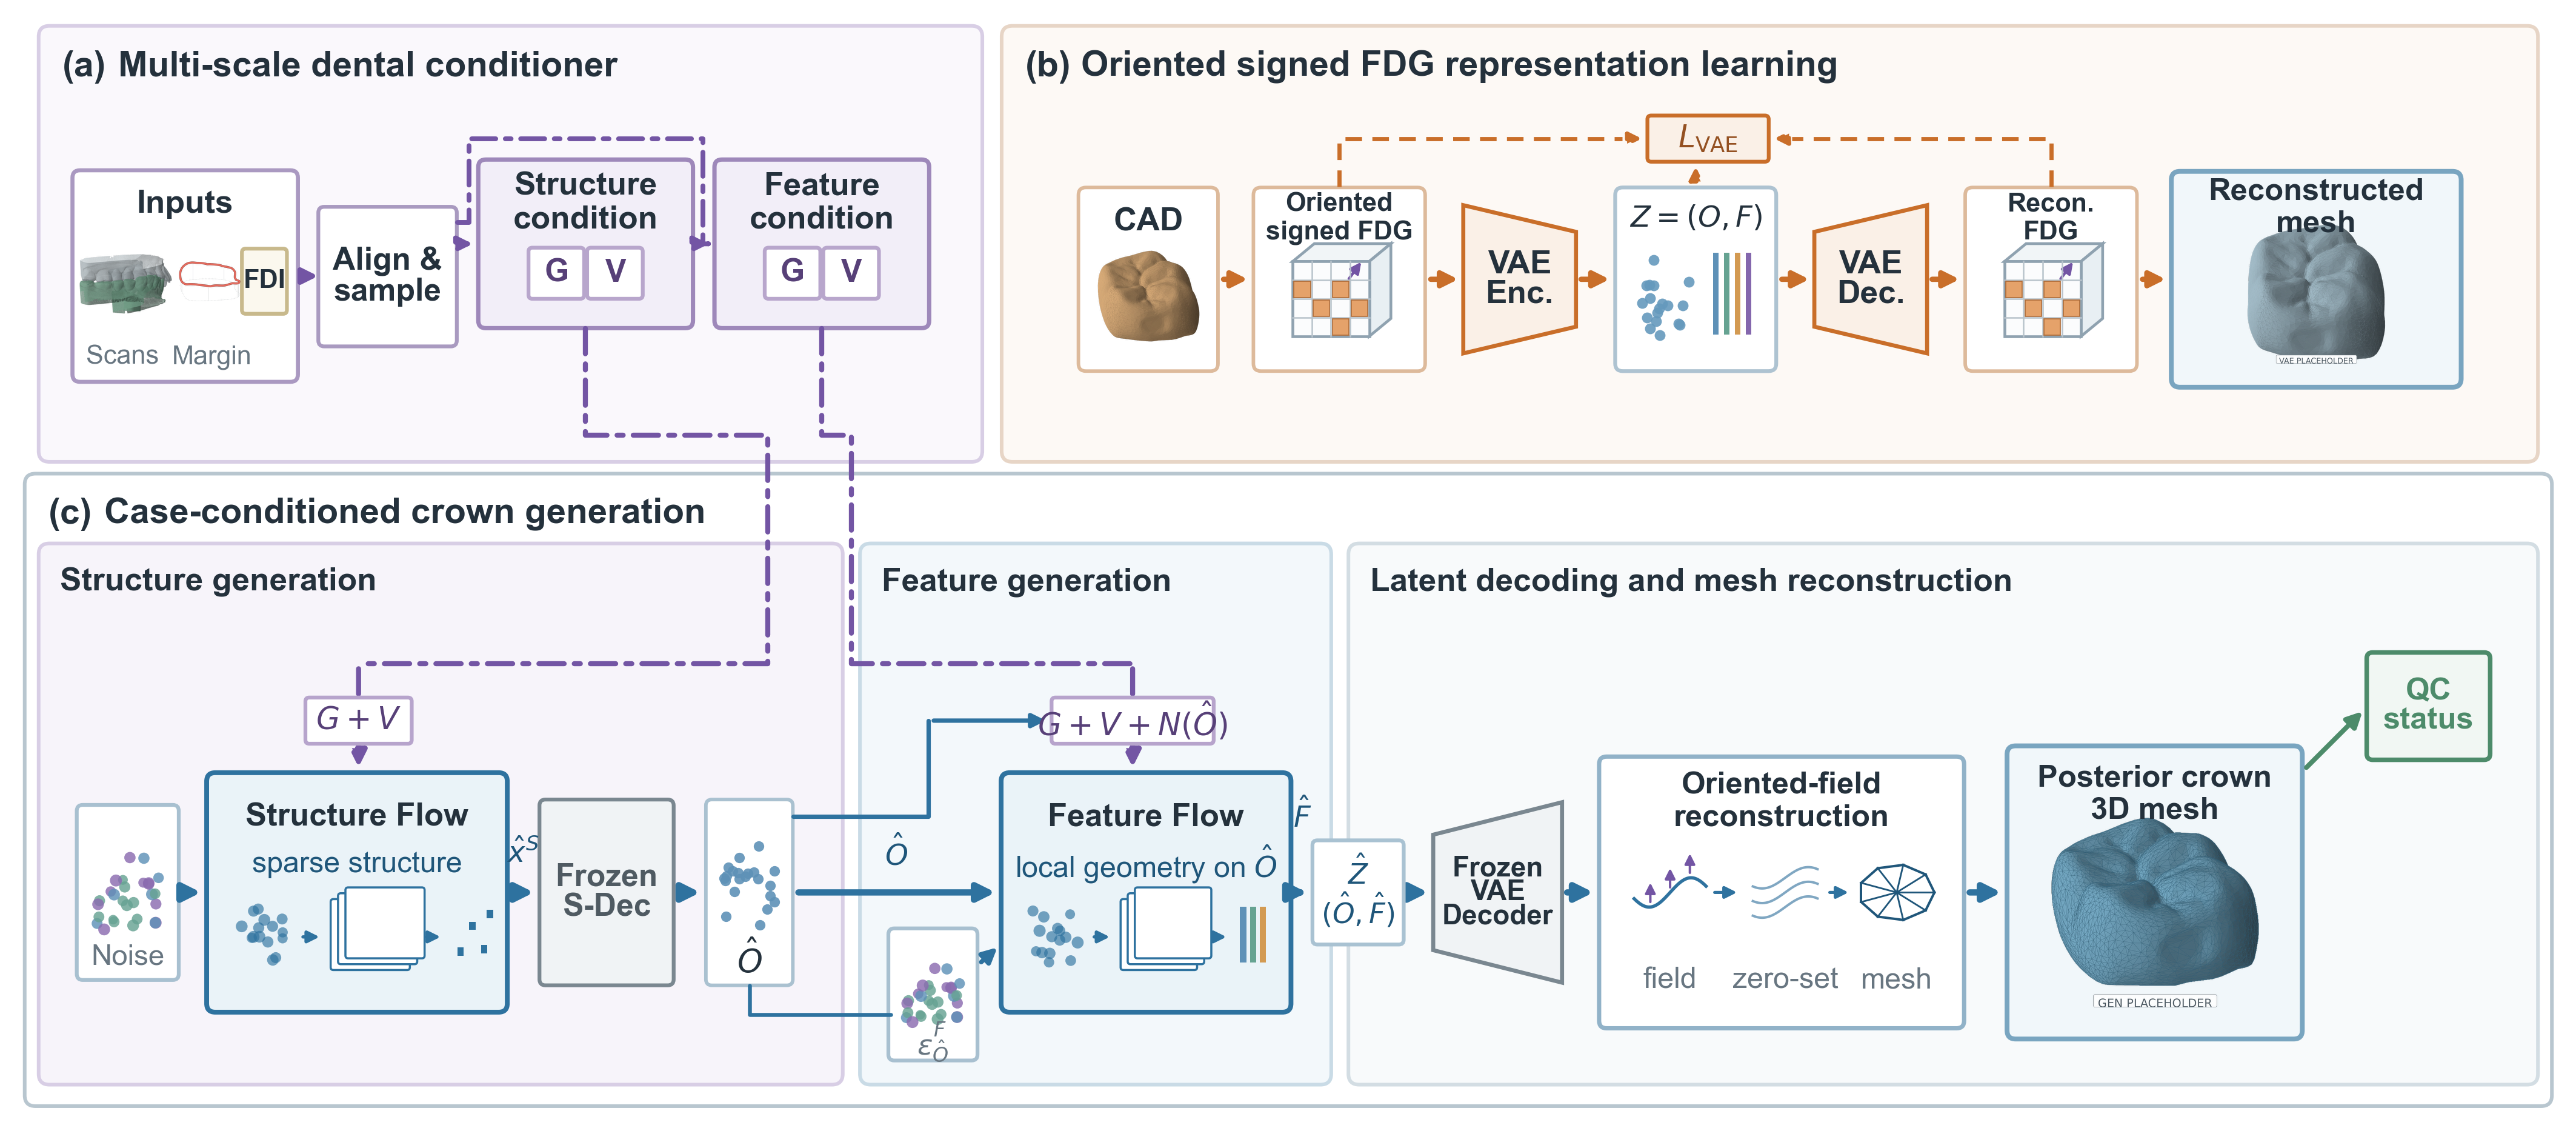
\includegraphics[width=1.0\textwidth]{./figures/method_framework.png}
    \caption{\textbf{Case-conditioned dental crown generation framework.} (a) After alignment and sampling, the maxillary and mandibular scans, three-dimensional cervical margin line, and FDI tooth designation are processed by two encoders with independent parameters to produce global and voxel-aligned conditions (\(G,V\)) for the Structure stage and the Feature-stage condition set \((G,V,N(\hat{O}))\), whose coordinate-neighborhood component is queried at the predicted support \(\hat{O}\). (b) The reference CAD model is converted into an oriented signed FDG and encoded into the latent representation \(Z=(O,F)\) by a trainable sparse VAE. The target and decoded FDGs provide reconstruction supervision, and a KL term regularizes the latent posterior; meshes reconstructed by standalone VAE decoding are used solely for visualization and evaluation. (c) Structure Flow generates a structural latent from noise, which is mapped by a frozen structure decoder to the predicted active support \(\hat{O}\). Given \(\hat{O}\) and noise defined over its active coordinates, Feature Flow generates local features \(\hat{F}\). The resulting latent \(\hat{Z}=(\hat{O},\hat{F})\) is decoded by the frozen VAE and reconstructed through a continuous oriented field to yield a candidate crown mesh, while an independent auxiliary branch reports the engineering-quality status. Purple dash-dotted lines denote dental conditioning, solid blue lines denote generation and support-dependency paths, and solid and dashed orange lines denote the VAE forward path and training supervision, respectively.}
    \label{fig:figure_overall_architecture} 
\end{figure*}

%% 3
\section{Method}\label{sec3}

%% 3.1
\subsection{Overview}\label{subsec3_1}

\hspace{2em}Figure~\ref{fig:figure_overall_architecture} presents the proposed case-conditioned crown generation framework with five components: input preprocessing and local coordinate construction, oriented signed FDG representation learning, multiscale dental conditioning, two-stage conditional flow matching, and oriented-field reconstruction with mesh extraction. The framework uses maxillary and mandibular scans, a 3D margin line, and an FDI tooth identifier as inputs, with reference CAD meshes as supervision to generate tooth-supported posterior single-crown meshes. In panel (a), the dental conditioner samples the dental arches and margin line, encodes the FDI identifier, and supplies $G$ and $V$ to both flows and $N(\hat{O})$ to Feature Flow. Panel (b) converts the reference CAD mesh into an oriented signed FDG, which the sparse VAE encodes as $Z=(O,F)$. In panel (c), Structure Flow generates $\hat{O}$, on which Feature Flow predicts $\hat{F}$. The resulting latent $\hat{Z}=(\hat{O},\hat{F})$ is decoded by the frozen VAE into the candidate crown mesh.

\hspace{2em}The proposed design preserves high-resolution crown geometry and surface orientation through a sparse representation, integrates tooth-position, interarch, and margin constraints via multiscale conditioning, and models global structure and local anatomy through two-stage generation. The following subsections detail each module.

%% 3.2
\subsection{Data Preprocessing and Local Coordinates}\label{subsec3_2}

\hspace{2em}This stage corresponds to input alignment and sampling in the left portion of Fig.~\ref{fig:figure_overall_architecture}(a). To remove inter-case variation in position and orientation, we construct a local orthonormal coordinate system from the margin line and dental arches. The origin \(o_i\) is defined as the mean of the margin points. The SVD direction associated with the smallest singular value of the centered margin points defines the candidate \(z\) axis; after identifying the target and opposing arches from the FDI tooth identifier, its sign is selected to point toward the mean of the nearest opposing-arch vertices. The \(y\) axis is obtained by normalizing the projection of the vector from the target-arch coordinate-wise median to \(o_i\) onto the plane orthogonal to \(z\); if this projection is degenerate, the first principal direction of the margin SVD is used. We then set \(x=y\times z\) and reorthogonalize \(y=z\times x\) to form the right-handed matrix \(A_i\), which maps world coordinates to local coordinates as \(T_i(p)=(p-o_i)A_i\). This transformation uses only the maxillary and mandibular scans, margin line, and FDI tooth identifier, without accessing the reference CAD; therefore, it introduces no target-geometry leakage during preprocessing.

\hspace{2em}After rigid alignment, the reference CAD mesh is discretized within a fixed physical domain with half-side length \(h=12\,\mathrm{mm}\). Vertices from the maxillary and mandibular meshes are used as candidates, prioritizing those near the margin centroid; if the local candidate set is insufficient, all vertices of the corresponding arch are used as a fallback. For each arch, 4,096 points with normals are randomly sampled, and the margin line is resampled to 1,024 points. The dental-arch and margin coordinates are normalized before encoder input, whereas normals are rotated, normalized, and set to zero when degenerate. Sampling randomness is determined by a fixed seed and the case-ID hash.

%% 3.3
\subsection{Oriented Signed FDG and Sparse Geometric VAE}\label{subsec3_3}

\hspace{2em}This module corresponds to the geometric representation and latent-space compression pathway in Fig.~\ref{fig:figure_overall_architecture}(b): the reference CAD mesh is first converted into an oriented signed FDG and then encoded by the sparse geometric VAE into the latent representation \(Z=(O,F)\).

%% 3.3.1
\subsubsection{Oriented Signed FDG}\label{subsubsec3_3_1}

\hspace{2em}The Flexible Dual Grid (FDG) stores geometric information only in active cells within the crown surface neighborhood, thereby avoiding construction of a dense high-resolution voxel grid [9]. For a grid of resolution \(R\), let \(c_j\in\{0,\ldots,R-1\}^3\) denote an active cell coordinate and \(\xi_j=c_j+0.5\) its center. The corresponding local physical coordinate is \(x_j=2h(\xi_j/R-0.5)\). Standard FDG encodes the within-cell offset of the dual-grid vertex, \(v_j\in[0,1]^3\), and three axial intersection indicators, \(b_j\in\{0,1\}^3\). Its nominal spacing, \(\Delta=2h/R\), specifies the discretization resolution rather than scan or clinical measurement accuracy.

\hspace{2em}Standard FDG represents local geometry and connectivity but does not explicitly encode the two sides of a surface or its orientation. We therefore augment it with a truncated signed distance and an oriented normal. Before nearest-surface queries, we repair inconsistent mesh winding, reverse watertight meshes with negative signed volume, and remove degenerate triangles. Let \(p_j\) be the closest point on the reference surface to \(x_j\), \(n_j^f\) the unit normal of the closest triangle, and \(n_j\) the barycentrically interpolated and normalized vertex normal at \(p_j\), set to zero in degenerate cases. The oriented truncated signed distance and normal feature are defined as
\[
\begin{aligned}
d_j&=\operatorname{clip}\!\left(
\operatorname{sign}\!\left[(x_j-p_j)^\top n_j^f\right]
\frac{\|x_j-p_j\|_2}{\Delta},-\tau,\tau
\right),\quad \tau=3,\\
g_j&=[v_j-0.5,\ b_j-0.5,\ d_j,\ n_j]\in\mathbb R^{10}.
\end{aligned}
\]
This representation jointly encodes local geometry, distance, and orientation within the sparse surface neighborhood. For watertight, consistently oriented meshes, the sign of \(d_j\) denotes global inside--outside status; for non-watertight meshes, it indicates only the local direction defined by the nearest surface normal. Fig.~2 illustrates the latent encoding of sparse active cells and their oriented signed attributes.

%% 3.3.2
\subsubsection{Sparse Geometric VAE}\label{subsubsec3_3_2}

\hspace{2em}The sparse geometric VAE compresses the high-resolution representation into a latent space suitable for generative modeling. Its five-level encoder has channel widths of 48, 96, 192, 384, and 512, with two encoding blocks per level. Four spatial-to-channel rearrangements reduce the active support at \(1024^3\) resolution to a 32-channel latent representation defined on a sparse \(64^3\) grid, where each active location predicts a 32-dimensional mean vector and log-variance vector. VAE training uses reparameterized sampling; the posterior mean is used for validation, free decoding, and Flow latent caching, whereas generation directly uses latents predicted by the Flow models. The symmetric decoder progressively predicts refinement masks and restores vertex offsets, axial-intersection logits, truncated signed distances, and normalized normals at the original resolution. It also predicts the quadrilateral triangulation weights required for differentiable FDG mesh extraction.

\begin{figure*}[t]  % [t] 表示尽量放在页面顶部
    \centering % 图片居中
    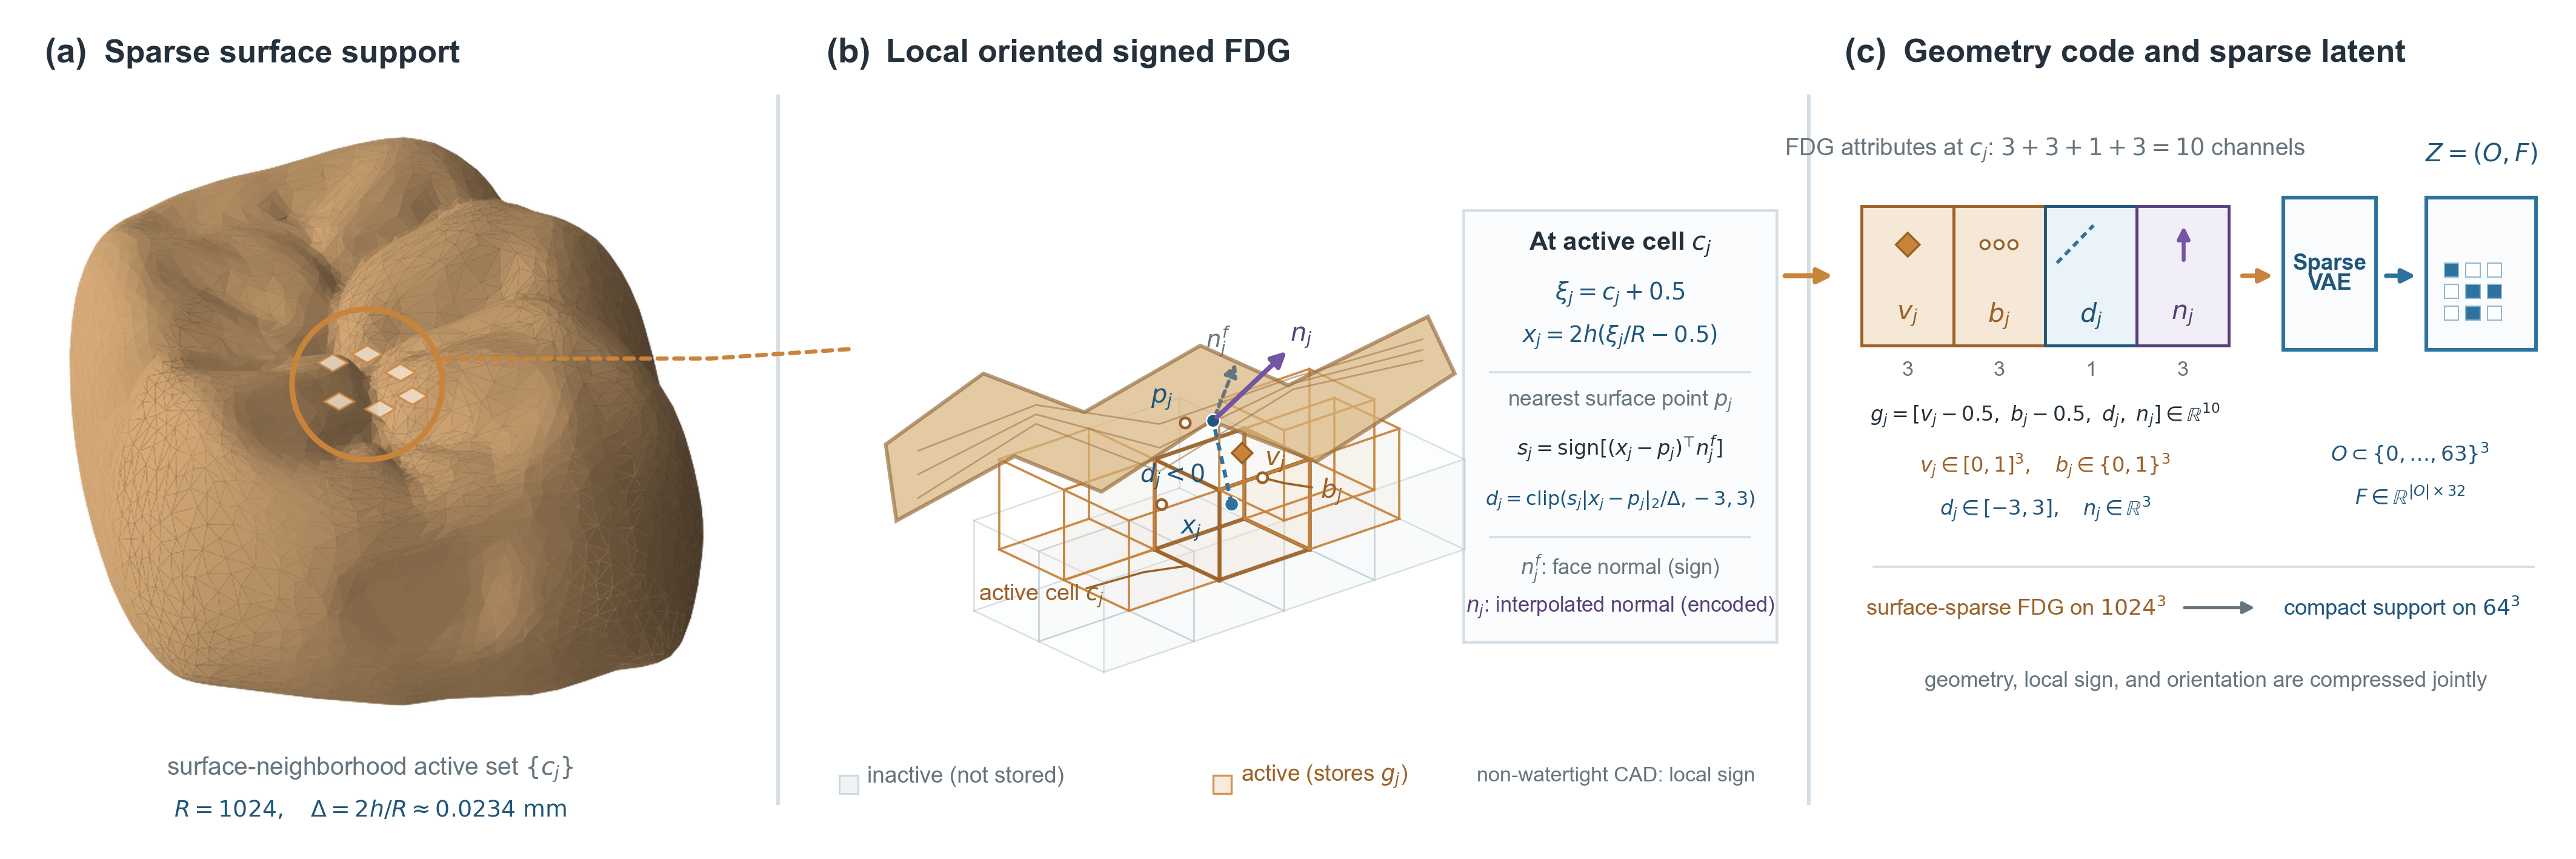
\includegraphics[width=1.0\textwidth]{./figures/oriented_signed_fdg_detail.png}
    \caption{\textbf{Sparse representation and latent encoding of the oriented signed FDG.} (a) The reference CAD activates only crown surface-neighborhood cells on an \(R=1024\) grid, with nominal spacing \(\Delta=2h/R\). (b) For each active coordinate \(c_j\), FDG records the vertex offset \(v_j\) and axis-aligned intersection flags \(b_j\). The cell center \(x_j\) queries the nearest surface point \(p_j\); the nearest-face normal \(n_j^f\) determines the local sign of the truncated signed distance \(d_j\), while the interpolated normal \(n_j\) provides oriented surface information. (c) The four attributes form \(g_j\in\mathbb{R}^{10}\) with \(3+3+1+3\) channels and are compressed by the sparse geometric VAE into 32-dimensional local features \(F\) defined on the \(64^3\) support \(O\). Inactive cells store no geometry; for non-watertight reference meshes, the sign of \(d_j\) denotes only the local orientation defined by the nearest-surface normal.}
    \label{fig:figure_ooriented_signed_fdg_detail} 
\end{figure*}


%% 3.4
\subsection{Attention-guided Fusion Module}\label{subsec3_4}

\hspace{2em}AFM serves as the critical integration component, dynamically integrating global and local features to address complex dental segmentation challenges. Fig. \ref{fig:fusion_module_architecture} illustrates its detailed architecture. Features from both branches are processed through a transformer-based mechanism, enabling adaptive feature weighting based on geometric contexts to handle diverse morphological variations in dental structures.

\begin{figure*}[t]
    \centering
    \includegraphics[width=0.7\textwidth, keepaspectratio]{aff_frame.pdf}
    \caption{Architecture of the proposed Attention-guided Fusion Module. The module takes local features, global features, and vertex positions as input, and outputs fused features that effectively combine local geometric details with global contextual information through dynamic attention mechanisms.}\label{fig:fusion_module_architecture}
\end{figure*}

\hspace{2em}The module takes three inputs: global features from the G Branch for overall shape understanding, local features from the L Branch for vertex-level geometric details, and 3D coordinates for geometry-aware position encoding. The AFM consists of three core components: Geometry-aware Position Encoding, Additive Feature Fusion, and Dynamic Multi-Head Attention, each described in detail below.

\bigskip

\textbf{Geometry-aware Position Encoding.} Standard Transformer architectures~\cite{hassija2025transformers} rely on self-attention mechanisms but inherently lack spatial awareness. Conventional position encoding methods, including sinusoidal functions and learned embeddings, are designed for sequential or grid-structured data and fail to capture the complex 3D spatial relationships essential for dental mesh analysis. To address this limitation, we propose a geometry-aware position encoding mechanism that directly leverages 3D vertex coordinates:

\begin{equation} \mathbf{P} = \mathbf{V} \mathbf{W}_{pos} + \mathbf{b}_{pos} \end{equation}

where $\mathbf{V} \in \mathbb{R}^{N \times 3}$ represents vertex coordinates, $\mathbf{W}_{pos} \in \mathbb{R}^{3 \times {d}_{G}}$ and $\mathbf{b}_{pos} \in \mathbb{R}^{{d}_{G}}$ are learnable position encoding parameters, $d_G$ is the global feature dimension. This formulation enables the model to learn geometric embeddings suited for complex dental surface representation.


% 伪代码
\begin{algorithm}[t]
    \SetAlgoLined
    \SetKwInOut{KwInput}{Input}
    \SetKwInOut{KwOutput}{Output}
    \SetKwInOut{KwParams}{Parameters}
    
    \caption{Attention-guided Fusion Module (AFM)}
    \label{alg:afm}
    \KwInput{$\mathbf{F}_L \in \mathbb{R}^{N \times d_L}$ (local feature), 
             $\mathbf{F}_G \in \mathbb{R}^{N \times d_G}$ (global feature), 
             $\mathbf{V} \in \mathbb{R}^{N \times 3}$ (vertex coordinate)}
    \KwOutput{$\mathbf{F}_{\text{out}} \in \mathbb{R}^{N \times C}$ (fused feature)}
    \KwParams{$h$ (initial number of attention heads, default $h=8$)}

    \tcp{Stage 1: Feature Projection and Geometry-aware Encoding (Corresponds to Fig. 4 left)}
    $\mathbf{P} \leftarrow \mathbf{V} \cdot \mathbf{W}_{\text{pos}} + \mathbf{b}_{\text{pos}}$ \tcp*{Geometry-aware position encoding}
    $\mathbf{F}_{\text{combined}} \leftarrow \mathbf{F}_L + \mathbf{F}_G + \mathbf{P}$ \tcp*{Additive feature fusion}
    
    \tcp{Stage 2: Dynamic Multi-Head Attention (Corresponds to Fig. 4 lower-right)}
    \eIf{$d_G \bmod h \neq 0$}{
        $h^* \leftarrow \max\left(1, \frac{d_G}{\lfloor d_G/h \rfloor + 1}\right)$ \tcp*{Dynamic head adjustment}
    }{
        $h^* \leftarrow h$ \tcp*{Use initial head count}
    }
    $d_h \leftarrow d_G / h^*$ \tcp*{Dimension per head}

    % $\mathbf{Q}, \mathbf{K}, \mathbf{V} \leftarrow \text{Linear}(\mathbf{F}_{\text{combined}}) \times 3$ \tcp*{Projections}
    \tcp{Linear projections for Q, K, V}
    $\mathbf{Q} \leftarrow \mathbf{F}_{\text{combined}} \mathbf{W}_Q, \quad \mathbf{K} \leftarrow \mathbf{F}_{\text{combined}} \mathbf{W}_K, \quad \mathbf{V} \leftarrow \mathbf{F}_{\text{combined}} \mathbf{W}_V$\;
    
    \tcp{Multi-head attention computation}
    \For{$i = 1$ \KwTo $h^*$}{
        $\text{Attn}_i \leftarrow \text{softmax}\left(\mathbf{Q}_i \mathbf{K}_i^\top / \sqrt{d_h}\right) \cdot \mathbf{V}_i$\;
    }
    $\mathbf{F}_{\text{attn}} \leftarrow \text{Concat}(\text{Attn}_1, \ldots, \text{Attn}_{h^*}) \cdot \mathbf{W}_O$\; 
    
    \tcp{Stage 3: Residual Connection and Feed-Forward (Corresponds to Fig. 4 right)}
    $\mathbf{F}_{\text{norm}} \leftarrow \text{LayerNorm}(\mathbf{F}_{\text{attn}} + \mathbf{F}_{\text{combined}})$ \tcp*{Residual + LayerNorm}
    $\mathbf{F}_{\text{ffn}} \leftarrow \text{Linear}_{\text{out}}(\text{ReLU}(\text{Linear}_{\text{in}}(\mathbf{F}_{\text{norm}})))$ \tcp*{Feed-Forward}
    $\mathbf{F}_{\text{out}} \leftarrow \text{LayerNorm}(\mathbf{F}_{\text{ffn}} + \mathbf{F}_{\text{norm}})$ \tcp*{Final residual + LayerNorm}
    
    \Return{$\mathbf{F}_{\text{out}}$}
\end{algorithm}


\textbf{Additive Feature Fusion.} An additive feature-fusion strategy is introduced for efficient integration of multi-source features while preserving dimensional consistency:

\begin{equation} \mathbf{F}_{combined} = \mathbf{F}_L + \mathbf{F}_G + \mathbf{P} \end{equation}

Here, $\mathbf{F}_L$, $\mathbf{F}_G$, and $\mathbf{P}$ denote the local feature, global feature, and position-encoded feature, respectively. Compared to concatenation-based fusion, the proposed strategy preserves feature dimensions while enabling direct channel-wise interaction and maintaining computational efficiency, thereby achieving an optimal balance between performance and cost without parameter inflation.

\bigskip

\textbf{Dynamic Multi-Head Attention.} The details of the module are shown in the lower-right corner of Fig. \ref{fig:fusion_module_architecture}. This module takes the fused feature $\mathbf{F}_{\text{combined}}$ as input and employs the standard attention mechanism. For each vertex $i$, we compute the query, key, and value vectors through linear projections:
\begin{equation}
\mathbf{Q}_i = \mathbf{F}_{\text{combined}}[i] \cdot \mathbf{W}_Q, \quad \mathbf{K}_i = \mathbf{F}_{\text{combined}}[i] \cdot \mathbf{W}_K, \quad \mathbf{V}_i = \mathbf{F}_{\text{combined}}[i] \cdot \mathbf{W}_V
\end{equation}
where $\mathbf{W}_Q, \mathbf{W}_K, \mathbf{W}_V \in \mathbb{R}^{d_G \times d_h}$ are learnable projection matrices, and $d_h$ denotes the dimension per attention head.

\hspace{2em}The core innovation lies in dynamically adjusting the number of attention heads $h^*$, based on the feature dimension $d_G$:
\begin{equation}
h^* = \max\left(1, \left\lfloor \frac{d_G}{h} \right\rfloor + 1\right) \quad \text{if } d_G \bmod h \neq 0
\end{equation}
where $h$ is the initial head count. This mechanism ensures that the number of attention heads is dynamically adjusted to maintain compatibility with the feature dimensions, optimizing computational efficiency and model performance.

\hspace{2em}The AFM dynamically balances contributions between global positional information and local geometric details, treating the centroid heatmap as a complementary prior. In complex dentitions such as crowded teeth, it adaptively refines coarse localization with boundary features, reducing centroid reliance when local boundaries indicate clearer separation, thereby resolving ambiguities and semantic inconsistencies. The detailed algorithmic procedure is summarized in Algorithm~\ref{alg:afm}.

%% 3.5
\subsection{Loss Function}\label{subsec3_5}

\hspace{2em}We introduce three efficient loss functions to further enhance performance, including centroid-guided loss \cite{zhao2024few}, local region loss, and boundary-constrained loss \cite{tan2023boundary}. These functions can effectively improve the accuracy and robustness of segmentation models.

\bigskip

\textbf{Centroid Guided Loss.} The centroid guided loss is designed to accurately locate tooth centroids. It is defined as:

\begin{equation} 
L_{centroid}=\frac{1}{N}\sum_{i=1}^N\left\|C_i-\hat{C}_i\right\|^2
\end{equation}
where \( N \) denotes the number of teeth. \( C_{i} \) corresponds to the reference centroid of the \( i-th \) tooth. While \(\hat{C}_{i}\) signifies the predicted centroid of the \( i-th \) tooth.

\bigskip

\textbf{Local Region Loss.} Local region loss focuses on precise segmentation within local regions. It is defined as:
\begin{equation}
L_{local}=\frac{1}{M}\sum_{j=1}^M\left(1-\frac{2\cdot TP_j}{TP_j+FP_j+FN_j}\right)
\end{equation}
where \( M \) is the number of local regions, \( TP_j \) refers to the true positive count for the \( j-th \) local region, \( FP_j \) denotes the false-positive count within the \( j-th \) local region, and \( FN_j \) denotes the false-negative count within the \( j-th \) local region.

\setlength{\parindent}{0pt}
\hspace{2em}This loss function aims to maximize the Dice coefficient within each local region, ensuring precise segmentation.

\bigskip

\textbf{Boundary-Constrained Loss.} The boundary-constrained loss ensures clear and accurate delineation of tooth boundaries. It is defined as
\begin{equation}
L_{boundary}=\frac{1}{K}\sum_{k=1}^K\left(1-\frac{\left|B_k\cap\hat{B}_k\right|}{\left|B_k\cup\hat{B}_k\right|}\right)
\end{equation}
where \( K \) is the number of boundaries, \( B_k \) is associated with the ground-truth boundary of the \( k-th \) tooth, and \(\hat{B}_{k}\) pertains to the predicted boundary of the \( k-th \) tooth.

\setlength{\parindent}{0pt}
\hspace{2em}This loss function minimizes the boundary distance between the predicted and true boundaries, ensuring accurate delineation.

\bigskip

\textbf{Final Loss Function.} The final loss function combines the above three losses with appropriate weights:
\begin{equation}
L_{final} = \alpha \cdot L_{centroid} + \beta \cdot L_{local} + \gamma \cdot L_{boundary}
\label{eq:final_loss}
\end{equation}
where \( \alpha \), \( \beta \) and \( \gamma \) are hyperparameters that balance the contributions of each loss function.

\setlength{\parindent}{0pt}

\hspace{2em}This comprehensive loss function ensures that the model achieves high accuracy in both centroid localization, local region segmentation, and boundary delineation. By integrating these complementary loss components, the model becomes more robust to variations in dental morphology and arrangement, effectively handling cases with complex tooth geometry. 

%% 4
\section{Experimental and Discussions}\label{sec4}

%% 4.1 
\subsection{Dataset}\label{subsec4_1}

\hspace{2em}In the course of our experiments, we made use of several public datasets with a view to assess PASegNet's performance. The Teeth3DS dataset \cite{ben2022teeth3ds}, with 1800 high-precision intraoral 3D scans, offers a comprehensive representation of diverse dental conditions, from normal to pathological, with detailed FDI notation-based annotations. Meanwhile, the 3DTeethSeg dataset \cite{ben20233dteethseg}, consisting of 900 high-resolution 3D dental meshes, provides sufficient tooth morphology variability to challenge segmentation algorithms. These datasets collectively cover a wide range of dental scenarios, including complex cases like missing teeth, severe misalignment, crowding, dental restorations, and anatomical anomalies. Following standard protocols, we randomly split the datasets into training (70\%), validation (15\%), and testing (15\%) sets, ensuring similar complex case distribution across all splits, thereby enabling a thorough evaluation of our method's robustness in various clinical situations.

%% 4.2 
\subsection{Evaluation metrics}\label{subsec4_2}

\hspace{2em}To assess the segmentation performance, we employed the following metrics:

\bigskip

\hspace{2em} \textbf{Overall Accuracy (OA):} \hspace{1em} OA is a metric used to evaluate the overall accuracy of tooth segmentation \cite{zhang2021tsgcnet}. It is defined as the ratio of correctly predicted grids to the total number of grids, expressed mathematically as:

\begin{equation}
\mathrm{OA}=\frac{N_{\mathrm{correct}}}{N_{\mathrm{total}}}
\end{equation}

where \( N_{correct} \) denotes the number of correctly predicted grids, and \( N_{total} \) represents the total number of grids. This metric reflects the model's general ability to segment accurately.

\bigskip

\hspace{2em} \textbf{Mean Intersection over Union (mIoU):} \hspace{1em}\( mIoU \)  is a measure of how well segmentation results match with ground truth annotations \cite{zhao2021two}. Its calculation formula is:

\begin{equation}
mIoU=\frac{1}{k+1}\sum_{i=0}^k\frac{p_{ii}}{\sum_{j=0}^kp_{ij}+\sum_{j=0}^kp_{ji}-p_{ii}}
\end{equation}

where \( k+1 \) represents the number of segmentation categories, \( p_{ij} \) denotes the probability that a grid predicted to belong to category i actually belongs to category j, and \( p_{ii} \) denotes the count of samples accurately predicted.

\bigskip

\hspace{2em} \textbf{Boundary Intersection over Union (B-IoU):} \hspace{1em}B-IoU is a metric specifically designed to evaluate the accuracy of tooth boundary segmentation, as referenced in \cite{cho2021weighted}. Its calculation formula is:

\begin{equation}
B\mathrm{-}IoU=\frac{\|A\cap B\|}{\|A\cup B\|}
\end{equation}

Here, \( A \) represents the predicted boundary points set, and \( B \) represents the ground truth boundary points set.

\setlength{\parindent}{0pt}
\hspace{2em}These formulas can help evaluate the performance of 3D tooth segmentation models, particularly in handling complex tooth arrangements and shape variations.

%% 4.3 
\subsection{Implementation Details}\label{subsec4_3}

\hspace{2em}Prior to training, all dental meshes undergo coordinate normalization: each mesh is centered at its centroid and scaled to fit within a unit sphere. This preprocessing ensures consistent scale across samples from different scanners and datasets, mitigating scale sensitivity. We adopted an end-to-end training approach to streamline the process and enable unified optimization. Specifically, the learning rate was initialized at $0.001$ with cosine annealing; the AdamW optimizer was employed with weight decay $0.01$; and a batch size of $8$ was selected to balance memory usage and stability. By combining optimized FPS sampling with this training strategy, PASegNet achieves practical efficiency for clinical 3D tooth segmentation.

\hspace{2em}For the loss function hyperparameters $\alpha$, $\beta$, and $\gamma$ in Eq.~\ref{eq:final_loss}, we conducted a systematic grid search on the validation set, exploring weight combinations in the range $[0.1, 1.0]$ with a step size of $0.1$. Each configuration was evaluated based on validation mIoU and B-IoU metrics. The final weights ($\alpha=0.3$, $\beta=0.4$, $\gamma=0.3$) were selected to balance centroid localization, regional accuracy, and boundary precision, with the slightly higher $\beta$ reflecting the importance of local region segmentation accuracy.

\hspace{2em}Systematic timing experiments on an NVIDIA RTX 3090 GPU demonstrate that PASegNet achieves an average inference time of 0.85 s per dental model (10,000 vertices) with only 4.2 GB GPU memory, enabling deployment on standard mid-range clinical workstations and real-time clinical applications. The architecture exhibits robust scalability across varying mesh resolutions (5,000 to 50,000 vertices), maintaining mIoU variance below 1.5\% with linear complexity relative to vertex count. This scalable AI infrastructure allows seamless integration into downstream clinical workflows, serving as a foundational segmentation engine for comprehensive digital dentistry solutions.

\begin{table*}[h]
    \captionsetup{
      justification=raggedright,
      singlelinecheck=false,
      margin=2.35cm    % ← 调整此值以和表格左边对齐
    }
    \caption{\\Performance comparison with state-of-the-art methods}\label{table_network_performance_compare}%
    \vspace{-8pt} 
    \centering
    \begin{tabular}{lccccc}
        \hline
        Method & OA(\%) & mIoU(\%) & B-IoU(\%) & Params(M) & FLOPs(G) \\ \hline
        DGCNN \cite{wang2019dynamic} & 85.72 & 76.43 & 69.22 & 3.5 & 3.8 \\
        IOSSAM \cite{huang2024iossam} & 87.89 & 84.23 & 78.15 & 9.2 & 14.8 \\
        SimpSegNet \cite{jana20233d} & 88.45 & 74.70 & 68.67 & 4.8 & 5.1 \\
        Geo-Net \cite{liu2024geo} & 88.76 & 80.91 & 80.45 & 10.2 & 5.8 \\
        CurSegNet \cite{mao2024cursegnet} & 89.12 & 81.45 & 81.67 & 2.6 & 2.5 \\
        TSegLab \cite{rekik2025tseglab} & 89.56 & 85.13 & 79.28 & 12.3 & 22.5 \\
        \textbf{Ours} & \textbf{90.98} & \textbf{93.68} & \textbf{82.56} & 5.8 & 5.3 \\ \hline
    \end{tabular}
\end{table*}

\begin{figure*}[t]
    \centering
    \includegraphics[width=1.0\textwidth]{merged_rendered_images.png}
    \caption{Visual evaluation of segmentation results across methods. Comparison between existing approaches and our PASegNet on representative dental cases. Our method demonstrates enhanced accuracy in challenging scenarios including crowded dentition, tooth misalignments, and complex morphologies.}\label{fig:figure_visual_segment_results}
\end{figure*}


%% 4.4
\subsection{Results and Analysis}\label{subsec4}

%% 4.4.1 Experiment Result
\subsubsection{Experiment Result}\label{subsubsec4_4_1}

\setlength{\parindent}{0pt}

\hspace{2em}To validate the effectiveness of our proposed method, we conducted a comprehensive comparative analysis against several state-of-the-art techniques. Considering the efficacy, domain relevance, and reproducibility of all listed approaches, the comparison included the following methods: DGCNN \cite{wang2019dynamic}, SimpSegNet \cite{jana20233d}, Geo-Net \cite{liu2024geo} and CurSegNet \cite{mao2024cursegnet}, TSegLab \cite{rekik2025tseglab}. The quantitative results are provided in Table \ref{table_network_performance_compare}. To ensure fair comparison, all methods were trained and evaluated under identical experimental conditions using the same datasets and preprocessing techniques. It is important to note that our evaluation focuses exclusively on the direct outputs from the neural networks without any post-processing steps or external auxiliary models. This approach allows for a more objective assessment of each model's intrinsic capabilities in handling the challenging task of 3D dental instance segmentation. As demonstrated in the results, our proposed PASegNet consistently outperforms existing methods across all evaluation metrics, particularly in handling complex dental morphologies.

% \begin{figure}[h]
%     \centering
%     \includegraphics[width=1.0\textwidth]{segmentation results.png}
%     \caption{Visualization of representative segmentation results comparing with four competing methods and our method.}\label{fig:figure5}
% \end{figure}


\hspace{2em}We also conducted qualitative experiments to assess the segmentation results shown in Fig. \ref{fig:figure_visual_segment_results}. Our method shows superior performance, especially in handling complex cases like wisdom teeth, crowded teeth, or misalignments. It accurately labels most teeth and effectively manages misaligned and worn teeth through semantics-guided segmentation and adaptive feature fusion. Additionally, our approach excels in local geometric feature extraction. These results confirm that our design is more effective and accurate for this segmentation task.

\begin{figure}[t]
    \centering
    \subfigure[Time Step: 0.001]{\includegraphics[width=0.35\linewidth]{combined_rendered_views_1t.png}}
    \subfigure[Time Step: 0.1]{\includegraphics[width=0.35\linewidth]{combined_rendered_views_2t.png}}
    \subfigure[Time Step: 10.0]{\includegraphics[width=0.35\linewidth]{combined_rendered_views_3t.png}}
    \subfigure[Time Step: 1000.0]{\includegraphics[width=0.35\linewidth]{combined_rendered_views_4t.png}}
    \caption{Visualization of heat diffusion at different timescales. The HKS features capture tooth boundary information with increasing diffusion over time, revealing detailed local geometry at small timescales (a) and broader structural information at larger timescales (d).}\label{fig:figure_diffusion_timestep}
\end{figure}

\begin{table}[h]
    \captionsetup{
      justification=raggedright,
      singlelinecheck=false,
      margin=4.6cm    % ← 调整此值以和表格左边对齐
    }
    \caption{\\Feature regions based on timescales}\label{tab:table_feature_timescales}
    \vspace{-8pt} 
    \centering
    \begin{tabular}{p{4.0cm}cc}
        \hline
        Feature Scale & Range \\ \hline
        Extremely Local Features & \( t \leq 0.01 \) \\
        Local Features & \( 0.01 < t \leq 1.0 \) \\
        Medium-Scale Features & \( 1.0 < t \leq 100.0 \) \\
        Global Features & \( t > 100.0 \) \\ \hline
    \end{tabular}
\end{table}

%% 4.4.2
\subsubsection{Ablation Study}\label{subsubsec4_4_2}

%%%% Ablation Study 1
\bigskip

\textbf{Effectiveness of the timescale parameter.} As shown in Fig. \ref{fig:figure_diffusion_timestep}, the timescale parameter is pivotal in HKS feature extraction and representation, as it governs the extent and intensity of heat diffusion. When the timescale is small, heat diffusion is confined to local regions, enabling HKS to capture delicate local geometric features such as edges and corners. As the timescale increases, the diffusion spreads to broader areas. Table \ref{tab:table_feature_timescales} details the relationship between timescale and feature regions. The timescale parameter is essential for achieving a balance between local and global information while maintaining stability and distinctiveness. In this scheme, the HKS focuses on local feature extraction, and the timescale is set to 0.01 to maintain computational efficiency.


\hspace{2em}The HKS features extracted by the BAM provide valuable local information, which serves as a complement to the global information captured by the position-aware Module (G branch). This merging of local and global context permits the model to attain more precise and stable segmentation outcomes.


%%%% Ablation Study 2
\bigskip

\textbf{Effectiveness of feature and architecture choices.} To validate our design choices, we conducted systematic ablation studies (Table~\ref{table_feature_representation}). For local geometric descriptors, HKS outperforms curvature by encoding multi-scale intrinsic geometry through heat diffusion, achieving a mIoU improvement of 4.76\% (93.68\% vs. 88.92\%). Additionally, HKS demonstrates superior robustness to scanning artifacts compared to WKS~\cite{aubry2011wave} due to its inherent smoothing property. For global feature architectures, EdgeConv outperforms both PointNeXt~\cite{qian2022pointnext} and Point Transformer V3 (PTv3)~\cite{wu2024point} through dynamic graph construction that adaptively captures local relationships, achieving the highest B-IoU of 82.56\% while maintaining computational efficiency suitable for clinical deployment. These results confirm that the combination of HKS and EdgeConv optimally balances segmentation accuracy and efficiency.

\begin{table*}[h]
    \captionsetup{
      justification=raggedright,
      singlelinecheck=false,
      margin=2.35cm    % ← 调整此值以和表格左边对齐
    }
    \caption{\\Ablation study on feature descriptors and architectures}\label{table_feature_representation}%
    \vspace{-8pt} 
    \centering
    \begin{tabular}{lcccc}
        \hline
        Local Feature & Global Architecture & OA(\%) & mIoU(\%) & B-IoU(\%) \\ \hline
        Curvature & EdgeConv  & 87.45 & 88.92 & 76.24 \\
        WKS       & EdgeConv  & 89.67 & 92.06 & 80.13 \\
        HKS       & PointNeXt & 89.12 & 91.35 & 79.85 \\
        HKS       & PTv3      & 90.67 & 93.41 & 81.78 \\
        \textbf{HKS(Ours)} & \textbf{EdgeConv(Ours)} & \textbf{90.98} & \textbf{93.68} & \textbf{82.56} \\ \hline
    \end{tabular}
\end{table*}

\bigskip

\textbf{Effectiveness of feature fusion module.} The feature fusion module is crucial for integrating local and global features. To evaluate the effectiveness of our method, we compared the proposed Attention-guided Fusion Module with several baseline methods, with the results in Table \ref{table_fusion_module_compare}. The experiments used the Teeth3DS \cite{ben2022teeth3ds} and 3DTeethSeg \cite{ben20233dteethseg} datasets, evaluating the OA and the mIoU. Baseline methods included simple concatenation, maximum pooling fusion, graph convolution fusion, and attention gating.

\hspace{2em}As shown in Table~\ref{table_fusion_module_compare}, both IoU and accuracy demonstrate progressive improvements with advancing fusion strategies. AFM effectively integrates global and local features through additive fusion that preserves feature dimensionality. Its dynamic attention-head mechanism further aligns computational complexity with $d_G$ without indiscriminately increasing parameters. Consequently, the observed performance gains are attributable to dual-branch complementarity rather than parameter-capacity inflation, thereby maintaining reasonable model complexity.

\begin{table*}[h]
    \captionsetup{
      justification=raggedright,
      singlelinecheck=false,
      margin=2.9cm    % ← 调整此值以和表格左边对齐
    }
    \caption{\\ Comparison of different feature fusion methods}\label{table_fusion_module_compare}
    \vspace{-8pt} 
    \centering
    \begin{tabular}{llll}
        \hline
        Method & OA~(\%) & mIoU~(\%) & Parameters \\ \hline
        Simple Concatenation        & 82.31 & 89.14 & 2.1M \\
        Maximum Pooling Fusion      & 83.27 & 90.52 & 1.8M \\
        Graph Convolution Fusion    & 85.41 & 91.57 & 3.2M \\
        Attention Gating Fusion     & 86.54 & 92.16 & 2.7M \\
        \textbf{Attention-guided Fusion (Ours)} & \textbf{90.98} & \textbf{93.68} & 2.4M \\ \hline
    \end{tabular}
\end{table*}

%%%% Ablation Study 3
\bigskip
\textbf{Effectiveness of dual-branch architecture.} To investigate the effectiveness of our dual-branch architecture and the contribution of HKS features to tooth boundary segmentation, we compared different network configurations. Table \ref{table_ablation_study} presents the quantitative results on both datasets, with particular focus on boundary segmentation accuracy measured by B-IoU.

\begin{table*}[t]
    \captionsetup{
      justification=raggedright,
      singlelinecheck=false,
      margin=2.35cm    % ← 调整此值以和表格左边对齐
    }
    \caption{\\ Ablation study on network architecture and feature representations}\label{table_ablation_study}%
    \vspace{-8pt} 
    \centering
    \begin{tabular}{p{4.0cm}cccc}
        \hline
        Method & OA (\%) & mIoU (\%) & B-IoU (\%) & Parameters \\ \hline
        DGCNN (single-branch) & 86.45 & 78.92 & 73.67 & 3.2M \\
        HKS (single-branch) & 87.32 & 80.14 & 75.23 & 3.5M \\
        \textbf{Dual-branch (Ours)} & \textbf{90.98} & \textbf{93.68} & \textbf{82.56} & 5.8M \\ \hline
        \multicolumn{5}{l}{\footnotesize \textit{Note: All methods trained on Teeth3DS dataset with identical settings.}} \\
    \end{tabular}
\end{table*}

\begin{figure}[H]
    \centering
    \subfigure[DGCNN]{\includegraphics[width=0.28\linewidth]{CombinedView_Ablation_Experiment2_1.png}}
    \subfigure[DGCNN + HKS]{\includegraphics[width=0.28\linewidth]{CombinedView_Ablation_Experiment2_2.png}}
    \subfigure[Ground truth]{\includegraphics[width=0.28\linewidth]{CombinedView_Ablation_Experiment2_3.png}}
    \caption{Comparison of tooth boundary segmentation results. (a) DGCNN (single-branch) shows inaccuracies at complex boundaries. (b) DGCNN + HKS (dual-branch) demonstrates improved boundary delineation. (c) Ground truth. The red circles highlight areas with challenging conditions.}\label{fig:figure_boundary_comparison}
\end{figure}

\begin{figure}[H]
    \centering
    \subfigure[HKS]{\includegraphics[width=0.28\linewidth]{CombinedView_Ablation_Experiment1_1.png}}
    \subfigure[DGCNN + HKS]{\includegraphics[width=0.28\linewidth]{CombinedView_Ablation_Experiment1_2.png}}
    \subfigure[Ground truth]{\includegraphics[width=0.28\linewidth]{CombinedView_Ablation_Experiment1_3.png}}
    \caption{Comparison of segmentation results for tooth area. (a) Single-branch HKS model showing segmentation errors in certain tooth regions. (b)  DGCNN + HKS (dual-branch) architecture with improved accuracy. (c) Ground truth segmentation. The red circles highlight areas with challenging conditions.}\label{fig:figure_toothnumer_comparison}
\end{figure}


\hspace{2em}The ablation results presented in Table \ref{table_ablation_study}, together with the visualizations in Fig. \ref{fig:figure_boundary_comparison} and Fig. \ref{fig:figure_toothnumer_comparison}, clearly demonstrate the complementary advantages of the proposed dual-branch architecture and the incorporation of HKS features. The baseline DGCNN (single-branch) model achieves reasonable overall accuracy; however, it exhibits limited boundary precision, particularly in regions with complex geometry or adjacent teeth, as reflected by a B-IoU of only 73.67\%. Introducing HKS features in a single-branch configuration enhances local boundary delineation (B-IoU increases to 75.23\%), but this approach remains susceptible to missing or misclassified tooth regions due to the absence of global contextual information. In contrast, the dual-branch architecture, which effectively integrates global contextual features from the position-aware branch with local geometric details from the boundary-aware branch, achieves superior performance (B-IoU 82.56\%, mIoU 93.68\%).

\begin{figure}[t]
    \centering
    \subfigure[Total Loss Curves]{\includegraphics[width=0.33\linewidth]{training_curves_1.png}}
    \subfigure[mIoU Curves] {\includegraphics[width=0.33\linewidth]{training_curves_2.png}}
    \subfigure[B-IoU Curves]{\includegraphics[width=0.33\linewidth]{training_curves_3.png}}
    \caption{Training performance of different loss functions. (a) Total Loss Curves show the "Final Loss" combination achieves the lowest loss. (b) mIoU Curves indicate "Final Loss" outperforms others by 5-8 percentage points. (c) B-IoU Curves reveal "Final Loss" and "Boundary Only" have better boundary detection. Integrating multiple losses improves segmentation accuracy.}\label{fig:figure_train_curves}
\end{figure}


\hspace{2em}As illustrated in Fig. \ref{fig:figure_boundary_comparison}, the dual-branch model yields clearer and more accurate tooth boundaries compared to single-branch baselines. Furthermore, Fig. \ref{fig:figure_toothnumer_comparison} demonstrates that the dual-branch approach not only improves boundary precision but also maintains global semantic consistency, thereby reducing errors such as missing or merged teeth. These findings confirm that the integration of global and local features is essential for achieving robust and high-quality 3D tooth segmentation in challenging clinical scenarios.


%%%% Ablation Study 4

\bigskip

\textbf{Effectiveness of different loss function.} To validate the effectiveness of different loss function combinations, we conducted ablation studies with four configurations: Centroid Only, Local Only, Boundary Only, and Final Loss, as shown in Fig. \ref{fig:figure_train_curves}. Results demonstrated significant differentiation: Centroid Only showed stable but limited performance (mIoU \~70\%); Local Only exhibited rapid early convergence but overfitting after 120 epochs; Boundary Only encountered training difficulties with plateau phases yet achieved superior boundary IoU (87\%); Final Loss displayed complex dynamics with initial instability during the first 40 epochs due to multi-objective optimization, followed by synergistic advantages in the intermediate phase, ultimately achieving optimal performance, validating the efficacy of collaborative multi-loss optimization.

%% 4.4.3 Discussion
\subsubsection{Discussion}\label{subsubsec4_4_3}

\hspace{2em}The superior performance of PASegNet can be attributed to its innovative dual-branch architecture and attention-guided fusion module. By integrating the position-aware branch that captures global spatial relationships between teeth with the boundary-aware branch that focuses on local geometric details, our approach achieves a more comprehensive understanding of dental morphology. The attention-guided feature fusion dynamically balances global contextual information with fine-grained local features, enabling more accurate segmentation in complex scenarios such as abnormal tooth positions and varying morphologies. This ability to simultaneously process global position information and local boundary details allows PASegNet to effectively handle challenging cases where conventional single-branch methods typically fail. Additionally, our novel loss functions further enhance the model's capability to accurately locate tooth centroids and delineate boundaries, contributing to the overall robustness of the segmentation results.

\hspace{2em}Despite promising results, PASegNet has limitations. Performance decreases with extremely crowded or severely malposed teeth, as shown in Fig. \ref{fig:figure_constraints_examples}. This is because the manner of cascading in the G-Branch cannot adapt well to the positioning of supernumerary teeth. Moreover, excessive tooth substance loss can also affect the algorithm's ability to localize teeth. While our approach effectively utilizes geometric features, current evaluation requires validation across more diverse populations and scanning devices. Future research should incorporate anatomical prior knowledge through pretraining, integrate multimodal imaging data sources \cite{tian2023survey,kot2025evolution,pan2025mdgformer}, and explore model compression for clinical settings. These steps will close the research-to-application gap and enhance the algorithm’s clinical usability.

%% 5
\section{Conclusion}\label{sec5}

\hspace{2em}We presented PASegNet, a novel dual-branch framework for 3D tooth instance segmentation that effectively addresses challenges in dental morphologies through its position-aware and boundary-aware branches. The innovative attention-guided feature fusion mechanism and specialized loss functions further enhance the model's performance by optimizing centroid localization and boundary delineation simultaneously. Experimental results demonstrate that our approach outperforms state-of-the-art methods in segmentation accuracy and boundary detection precision. The clinical impact of PASegNet extends beyond technical improvements. By providing accurate and automated tooth segmentation, it can simplify orthodontic workflows, accelerate treatment planning, and enable more precise interventions. As a fundamental algorithm, PASegNet can serve as a basis for various dental design software applications, including automatic tooth arrangement, computer-aided diagnosis, and orthodontic treatment monitoring, positioning it to play a significant role in advancing automated analysis of 3D dental models for clinical applications.



\bibliographystyle{elsarticle-num} 
\bibliography{sn-bibliography}% common bib file

\end{document}

\endinput
%%
%% End of file `main.tex'.